\FloatBarrier
\subsection{Log Analysis}
\label{appendix:log-analysis}
This section presents the descriptive results of the log analysis part
of the developer survey. Seven respondents completed the log analysis
questions ($n=7$). Three additional survey participants did not answer
this section. Unless stated otherwise, all results in this subsection
refer to these seven respondents.

\begin{figure}[H]
    \centering
    \scriptsize
    \begin{minipage}[t]{0.48\textwidth}
        \centering
        \textbf{\scriptsize
        What percentage of your overall time do you spend analysing data?}
        \vspace{0.15em}
        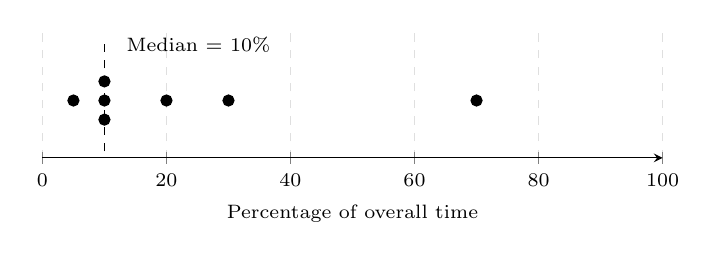
\begin{tikzpicture}
            \begin{axis}[
                width=0.78\linewidth,
                height=3.2cm,
                xmin=0,
                xmax=100,
                ymin=0.82,
                ymax=1.22,
                xtick={0,20,40,60,80,100},
                xlabel={Percentage of overall time},
                xlabel style={font=\scriptsize},
                tick label style={font=\scriptsize},
                ytick=\empty,
                axis y line=none,
                axis x line=bottom,
                grid=major,
                grid style={dashed,gray!25},
                clip=false
            ]
            \addplot[
                only marks,
                mark=*,
                mark size=2pt
            ] coordinates {
                (5,1.00)
                (10,0.94)
                (10,1.00)
                (10,1.06)
                (20,1.00)
                (30,1.00)
                (70,1.00)
            };
            \draw[dashed]
                (axis cs:10,0.84) --
                (axis cs:10,1.20);
            \node[
                anchor=south west,
                font=\scriptsize
            ] at (axis cs:12,1.12)
            {Median = 10\%};
            \end{axis}
        \end{tikzpicture}
        \par
        {\scriptsize
        (a) Overall time spent analysing logged data.}
    \end{minipage}\hfill%
    \begin{minipage}[t]{0.48\textwidth}
        \centering
        \textbf{\scriptsize
        Why do you analyze logged data?}
        \vspace{0.15em}
        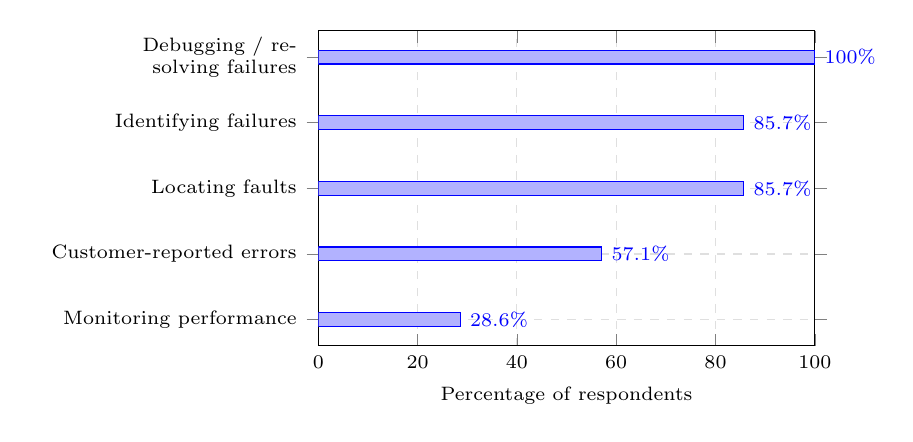
\begin{tikzpicture}
            \begin{axis}[
                xbar,
                width=0.52\linewidth,
                height=4.0cm,
                scale only axis,
                xmin=0,
                xmax=100,
                xtick={0,20,40,60,80,100},
                xlabel={Percentage of respondents},
                xlabel style={font=\scriptsize},
                symbolic y coords={
                    {Monitoring performance},
                    {Customer-reported errors},
                    {Locating faults},
                    {Identifying failures},
                    {Debugging / resolving failures}
                },
                ytick=data,
                yticklabel style={
                    text width=3.3cm,
                    align=right,
                    font=\scriptsize
                },
                tick label style={font=\scriptsize},
                nodes near coords={
                    \pgfmathprintnumber[fixed,precision=1]
                    {\pgfplotspointmeta}\%
                },
                every node near coord/.append style={
                    font=\scriptsize
                },
                point meta=x,
                bar width=5pt,
                enlarge y limits=0.10,
                grid=major,
                grid style={dashed,gray!25}
            ]
            \addplot coordinates {
                (28.6,{Monitoring performance})
                (57.1,{Customer-reported errors})
                (85.7,{Locating faults})
                (85.7,{Identifying failures})
                (100,{Debugging / resolving failures})
            };
            \end{axis}
        \end{tikzpicture}
        \par
        {\scriptsize
        (b) Reasons for analysing logged data.
        Multiple selections were possible.}
    \end{minipage}

    \par\vspace{0.35cm}

    \begin{minipage}[t]{0.48\textwidth}
        \centering
        \textbf{\scriptsize
        What log format do you primarily analyze?}
        \vspace{0.15em}
        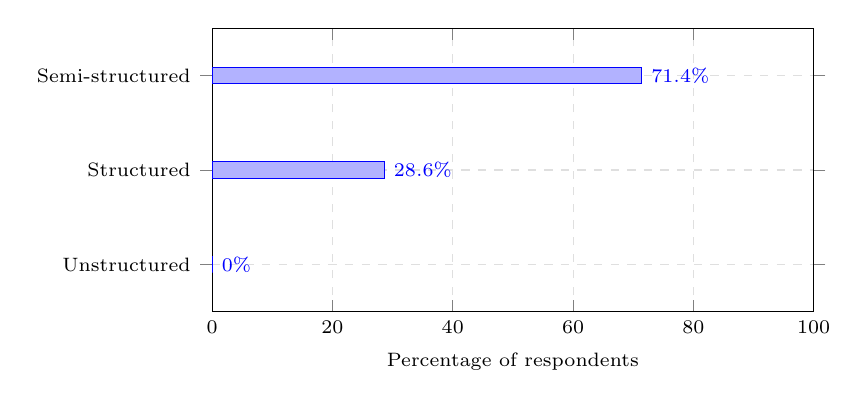
\begin{tikzpicture}
            \begin{axis}[
                xbar,
                width=0.63\linewidth,
                height=3.6cm,
                scale only axis,
                xmin=0,
                xmax=100,
                xtick={0,20,40,60,80,100},
                xlabel={Percentage of respondents},
                xlabel style={font=\scriptsize},
                symbolic y coords={
                    {Unstructured},
                    {Structured},
                    {Semi-structured}
                },
                ytick=data,
                yticklabel style={
                    font=\scriptsize
                },
                tick label style={font=\scriptsize},
                nodes near coords={
                    \pgfmathprintnumber[fixed,precision=1]
                    {\pgfplotspointmeta}\%
                },
                every node near coord/.append style={
                    font=\scriptsize
                },
                point meta=x,
                bar width=6pt,
                enlarge y limits=0.25,
                grid=major,
                grid style={dashed,gray!25}
            ]
            \addplot coordinates {
                (0,{Unstructured})
                (28.6,{Structured})
                (71.4,{Semi-structured})
            };
            \end{axis}
        \end{tikzpicture}
        \par
        {\scriptsize
        (c) Primary log format analyzed.}
    \end{minipage}\hfill%
    \begin{minipage}[t]{0.48\textwidth}
        \centering
        \textbf{\scriptsize
        How often do you perform the following log analysis activities?}
        \vspace{0.15em}
        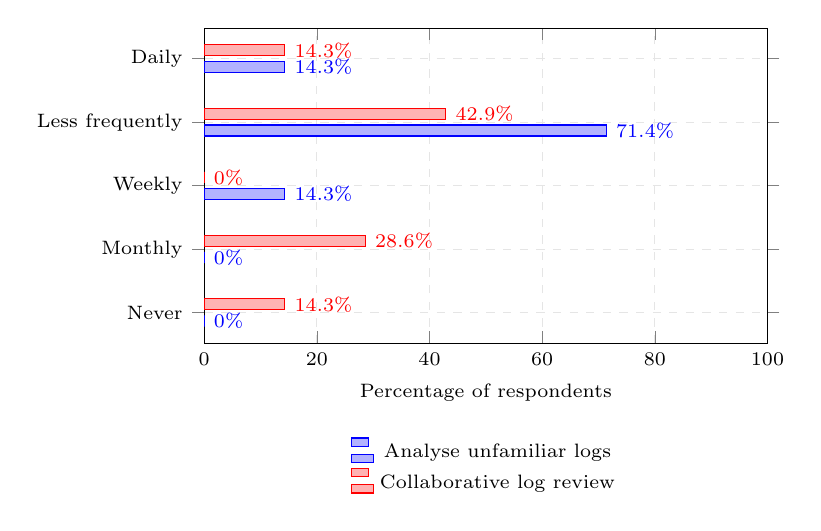
\begin{tikzpicture}
            \begin{axis}[
                xbar,
                width=0.59\linewidth,
                height=4.0cm,
                scale only axis,
                xmin=0,
                xmax=100,
                xtick={0,20,40,60,80,100},
                xlabel={Percentage of respondents},
                xlabel style={font=\scriptsize},
                symbolic y coords={
                    {Never},
                    {Monthly},
                    {Weekly},
                    {Less frequently},
                    {Daily}
                },
                ytick=data,
                yticklabel style={
                    font=\scriptsize
                },
                tick label style={font=\scriptsize},
                nodes near coords={
                    \pgfmathprintnumber[fixed,precision=1]
                    {\pgfplotspointmeta}\%
                },
                every node near coord/.append style={
                    font=\scriptsize
                },
                point meta=x,
                bar width=4pt,
                enlarge y limits=0.12,
                legend style={
                    at={(0.5,-0.28)},
                    anchor=north,
                    legend columns=1,
                    font=\scriptsize,
                    draw=none
                },
                grid=major,
                grid style={dashed,gray!20}
            ]
            % Analysis of unfamiliar logs
            \addplot coordinates {
                (0,{Never})
                (0,{Monthly})
                (14.3,{Weekly})
                (71.4,{Less frequently})
                (14.3,{Daily})
            };
            % Collaborative log review
            \addplot coordinates {
                (14.3,{Never})
                (28.6,{Monthly})
                (0,{Weekly})
                (42.9,{Less frequently})
                (14.3,{Daily})
            };
            \legend{
                Analyse unfamiliar logs,
                Collaborative log review
            }
            \end{axis}
        \end{tikzpicture}
        \par
        {\scriptsize
        (d) Frequency of selected log analysis activities.}
    \end{minipage}
    \caption{Selected descriptive results for log analysis.}
    \label{fig:appendix-log-analysis-overview}
\end{figure}

\clearpage

\begin{figure}[H]
    \centering
    \textbf{\scriptsize
    To which extent do you agree or disagree with the following
    statements?}
    \vspace{0.2em}
    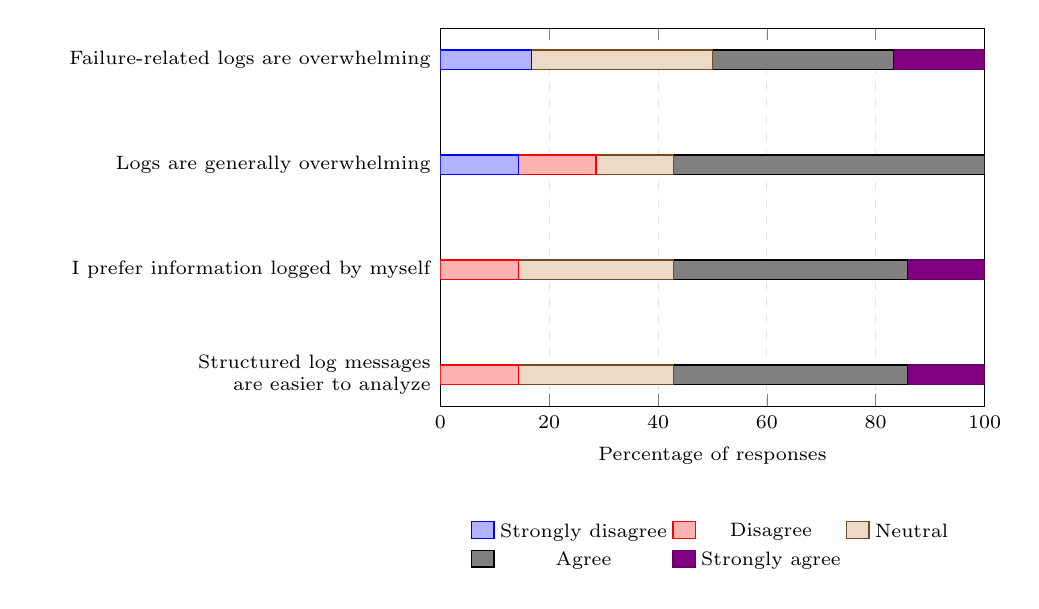
\begin{tikzpicture}
        \begin{axis}[
            xbar stacked,
            width=0.57\textwidth,
            height=4.8cm,
            scale only axis,
            xmin=0,
            xmax=100,
            xtick={0,20,40,60,80,100},
            xlabel={Percentage of responses},
            xlabel style={font=\scriptsize},
            symbolic y coords={
                {Structured log messages are easier to analyze},
                {I prefer information logged by myself},
                {Logs are generally overwhelming},
                {Failure-related logs are overwhelming}
            },
            ytick=data,
            yticklabel style={
                text width=5.0cm,
                align=right,
                font=\scriptsize
            },
            tick label style={font=\scriptsize},
            bar width=7pt,
            enlarge y limits=0.10,
            legend style={
                at={(0.5,-0.28)},
                anchor=north,
                legend columns=3,
                font=\scriptsize,
                draw=none
            },
            grid=major,
            grid style={dashed,gray!20}
        ]
        % Strongly disagree
        \addplot coordinates {
            (0,{Structured log messages are easier to analyze})
            (0,{I prefer information logged by myself})
            (14.3,{Logs are generally overwhelming})
            (16.7,{Failure-related logs are overwhelming})
        };
        % Disagree
        \addplot coordinates {
            (14.3,{Structured log messages are easier to analyze})
            (14.3,{I prefer information logged by myself})
            (14.3,{Logs are generally overwhelming})
            (0,{Failure-related logs are overwhelming})
        };
        % Neutral
        \addplot coordinates {
            (28.6,{Structured log messages are easier to analyze})
            (28.6,{I prefer information logged by myself})
            (14.3,{Logs are generally overwhelming})
            (33.3,{Failure-related logs are overwhelming})
        };
        % Agree
        \addplot coordinates {
            (42.9,{Structured log messages are easier to analyze})
            (42.9,{I prefer information logged by myself})
            (57.1,{Logs are generally overwhelming})
            (33.3,{Failure-related logs are overwhelming})
        };
        % Strongly agree
        \addplot coordinates {
            (14.3,{Structured log messages are easier to analyze})
            (14.3,{I prefer information logged by myself})
            (0,{Logs are generally overwhelming})
            (16.7,{Failure-related logs are overwhelming})
        };
        \legend{
            Strongly disagree,
            Disagree,
            Neutral,
            Agree,
            Strongly agree
        }
        \end{axis}
    \end{tikzpicture}
    \caption{Respondents' perceptions of log analysis. The statement
    concerning failure-related logs is based on six responses due to
    one missing answer; the remaining statements are based on seven
    responses.}
    \label{fig:appendix-log-analysis-perceptions}
\end{figure}

\vspace{-0.4em}
{\footnotesize
\noindent
\textbf{How do you typically access logs? Rank the methods below from
most often to least often.}
\smallskip
\noindent
None of the respondents provided a ranking for the listed log access
methods. Therefore, no quantitative ranking is presented for this
question.
}

\vspace{0.5em}
\subsubsection{Open-Ended Log Analysis Responses}
\label{appendix:open-ended-log-analysis}
{\footnotesize
The following tables present lightly paraphrased versions of the
open-ended survey responses. The responses were rephrased for
readability and conciseness while preserving their original meaning.
No additional thematic coding was applied.
}
\vspace{0.2em}

\begingroup
\scriptsize
\renewcommand{\arraystretch}{0.92}
\setlength{\tabcolsep}{4pt}
\begin{longtable}{
    @{}
    >{\centering\arraybackslash}p{0.04\textwidth}
    >{\RaggedRight\arraybackslash}p{0.43\textwidth}
    >{\RaggedRight\arraybackslash}p{0.47\textwidth}
    @{}
}
\caption{Paraphrased responses concerning log selection and the
analytical process.}
\label{tab:appendix-log-analysis-process}
\\\\
\toprule
\textbf{ID} &
\textbf{How do you know which logs to look at?} &
\textbf{Analytical process} \\\\
\midrule
\endfirsthead

\multicolumn{3}{l}{
    \scriptsize\textit{Table continued from previous page}
}
\\\\[0.15em]
\toprule
\textbf{ID} &
\textbf{How do you know which logs to look at?} &
\textbf{Analytical process} \\\\
\midrule
\endhead

\midrule
\multicolumn{3}{r}{
    \scriptsize\textit{Continued on next page}
}
\\\\
\endfoot

\bottomrule
\endlastfoot

P1 &
Recent logs associated with a build or operation that resulted in an
error are examined. &
Find the relevant log, search for the error, inspect the corresponding
source code, understand the cause, apply a fix, and rerun the software.
\\\\[0.15em]

P2 &
Relevant logs are selected based on previous experience. &
Understand the customer's reported problem and inspect the corresponding
logs for relevant details.
\\\\[0.15em]

P3 &
The affected component is first understood and the corresponding log
output path is identified in the source code. &
Read the log, trace the corresponding code, understand the code flow,
and identify the issue or error.
\\\\[0.15em]

P4 &
Logs from the most recent experiment are usually examined. For software
developed by others, the developer or documentation may be consulted. &
Locate the most recent error or warning message and follow it through
the code in a manner similar to following a stack trace.
\\\\[0.15em]

P5 &
Relevant logs are identified using their naming syntax. &
Use the timestamp and fault location and perform a text search for the
relevant information.
\\\\[0.15em]

P6 &
Logs are searched specifically for strings containing \texttt{error}. &
Copilot is primarily used for analysis. Previously, documentation and
interpretation of error codes were used.
\\\\[0.15em]

P7 &
The relevant log is selected based on the source of the problem; in
many cases the respondent already knows which log is most important. &
Examine system behaviour and how data changes over time to identify
unexpected or missing input and output data.
\\\\
\end{longtable}
\endgroup

\vspace{-0.4em}
\begingroup
\scriptsize
\renewcommand{\arraystretch}{0.92}
\setlength{\tabcolsep}{3pt}
\begin{longtable}{
    @{}
    >{\centering\arraybackslash}p{0.035\textwidth}
    >{\RaggedRight\arraybackslash}p{0.27\textwidth}
    >{\RaggedRight\arraybackslash}p{0.30\textwidth}
    >{\RaggedRight\arraybackslash}p{0.34\textwidth}
    @{}
}
\caption{Paraphrased open-ended responses concerning collaboration,
difficulties, and recommended log analysis practices.}
\label{tab:appendix-log-analysis-open-responses}
\\\\
\toprule
\textbf{ID} &
\textbf{Colleague involvement} &
\textbf{Issues or difficulties} &
\textbf{Recommended practices} \\\\
\midrule
\endfirsthead

\multicolumn{4}{l}{
    \scriptsize\textit{Table continued from previous page}
}
\\\\[0.15em]
\toprule
\textbf{ID} &
\textbf{Colleague involvement} &
\textbf{Issues or difficulties} &
\textbf{Recommended practices} \\\\
\midrule
\endhead

\midrule
\multicolumn{4}{r}{
    \scriptsize\textit{Continued on next page}
}
\\\\
\endfoot

\bottomrule
\endlastfoot

P1 &
Colleagues become involved when important components fail,
particularly where the respondent has previously worked. &
Different log structures can make logs difficult to understand. &
Use clear and well-structured logs and, where possible, a consistent
standard format.
\\\\[0.15em]

P2 &
Colleagues are involved only when additional developer-level support
is required. &
No particular difficulties were reported. &
No particular strategy was reported.
\\\\[0.15em]

P3 &
Team members use the logs to identify issues and support debugging. &
Understanding the code flow may remain difficult even after tracing
the corresponding log. &
Understand the relevant component and execution flow and analyse the
logs to identify abnormal behaviour.
\\\\[0.15em]

P4 &
Colleagues are rarely involved; when collaboration occurs, it is
similar to pair programming. &
Log messages are particularly difficult to use when they do not
indicate where the message originated. &
Perform log analysis diligently and in a structured manner.
\\\\[0.15em]

P5 &
Colleagues participate within the scope of their programming
responsibilities. &
Cryptic descriptions and missing information, such as timestamps,
make analysis difficult. &
Use text search and note frequently occurring or relevant keywords.
\\\\[0.15em]

P6 &
Other colleagues are involved when the respondent does not understand
a log entry. &
The main difficulty is identifying the root cause of a failure. &
No particular strategy was reported.
\\\\[0.15em]

P7 &
The issue is discussed collaboratively to determine the expected or
correct behaviour of the system. &
Identifying the correct timestamp can be difficult. &
Format logs so that important information is clearly highlighted and
easy to identify.
\\\\
\end{longtable}
\endgroup

\FloatBarrier
\clearpage
